\documentclass{article}
\usepackage{polski}
\usepackage[utf8]{inputenc}
\usepackage{listings}  
\usepackage{algpseudocode,algorithm,algorithmicx}
\usepackage{graphicx}
\usepackage{amsfonts}
\usepackage{amsmath}

\title{\textbf{Sprawozdanie}
\\\large Obliczenia naukowe 2019/2020 - lista 5}
\author{Tomasz Janik}
\date{}

\usepackage{natbib}
\usepackage{graphicx}

\usepackage{geometry}
 \geometry{
 a4paper,
 total={170mm,257mm},
 left=30mm,
 right=30mm,
 top=20mm,
 bottom=20mm
 }

\begin{document}
\maketitle
\section{Eliminacja Gaussa}

\subsection{Opis problemu}
Należało tutaj napisać funckję rozwiązującą metodą Gaussa układ równań w postaci:
\begin{center}
    $\mathbf{A}\mathbf{x} = \mathbf{b} $
\end{center}
z lub bez wyboru elementu głównego, dla danej macierzy współczynników $\mathbf{A} \in \mathbb{R}^{n \times n}$ i wektora prawych stron $\mathbf{b} \in \mathbb{R}^{n}$, n $\ge{4}$. Macierz $\mathbf{A}$ jest macierzą rzadką i blokową o następującej strukturze:
\begin{center}
    $$
    \mathbf{A} = 
    \begin{pmatrix}
        \mathbf{A}_{1} & \mathbf{C}_{1} & \mathbf{0} & \mathbf{0} & \mathbf{0} & \ldots & \mathbf{0} \\
        \mathbf{B}_{2} & \mathbf{A}_{2} & \mathbf{C}_{2} & \mathbf{0} & \mathbf{0} & \ldots & \mathbf{0} \\
        \mathbf{0} & \mathbf{B}_{3} & \mathbf{A}_{3} & \mathbf{C}_{3} & \mathbf{0} & \ldots & \mathbf{0} \\
        \vdots & \ddots & \ddots & \ddots & \ddots & \ddots & \vdots \\
        \mathbf{0} & \ldots & \mathbf{0} & \mathbf{B}_{v-2} & \mathbf{A}_{v-2} & \mathbf{C}_{v-2} & \mathbf{0} \\
        \mathbf{0} & \ldots & \mathbf{0} & \mathbf{0} & \mathbf{B}_{v-1} & \mathbf{A}_{v-1} & \mathbf{C}_{v-1} \\
        \mathbf{0} & \ldots & \mathbf{0} & \mathbf{0} & \mathbf{0} & \mathbf{B}_{v} & \mathbf{A}_{v} \\
    \end{pmatrix},
    $$
\end{center}
gdzie $v = \frac{n}{l}$, zakładając, że $n$ jest podzielne przez $l$, gdzie $l \ge{2}$ jest rozmiarem wszystkich kwadratowych macierzy wewnętrznych (bloków): $\mathbf{A}_{k}$, $\mathbf{B}_{k}$, $\mathbf{C}_{k}$. Mianowicie, $\mathbf{A}_{k} \in \mathbb{R}^{l \times l}$, $k = 1, \ldots, v$ jest macierzą gęstą, $\mathbf{0}$ jest kwadratową macierzą zerową stopnia $l$, macierz $\mathbf{B}_{k} \in \mathbb{R}^{l \times l}$, $k = 2, \ldots, v$ jest następującej postaci:
\begin{center}
    $$
    \mathbf{B}_{k} = 
    \begin{pmatrix}
        0 & \ldots & 0 & b_{1l-1}^{k} & b_{1l}^{k} \\
        0 & \ldots & 0 & b_{2l-1}^{k}  & b_{2l}^{k} \\    
        \vdots &  & \vdots & \vdots & \vdots \\
        0 & \ldots & 0 & b_{ll-1}^{k} & b_{ll}^{k} \\    
    \end{pmatrix},
    $$
\end{center}
$\mathbf{B}_{k}$ ma tylko dwie ostatnie kolumny niezerowe. Natomiast macierz $\mathbf{C}_{k} \in \mathbb{R}^{l \times l}$, $k = 1, \ldots, v - 1$ jest macierzą diagonalną:
\begin{center}
    $$
    \mathbf{C}_{k} = 
    \begin{pmatrix}
        c_{1}^{k} & 0 & 0 & \ldots & 0 \\
        0 & c_{2}^{k} & 0 & \ldots & 0 \\
        \vdots & \ddots & \ddots & \ddots & \vdots \\
        0 & \ldots & 0 & c_{l-1}^{k} & 0 \\
        0 & \ldots & 0 & 0 & c_{l}^{k} \\
    \end{pmatrix}.
    $$
\end{center}

\subsection{Metoda eliminacji Gaussa}
Eliminacja Gaussa polega na sprowadzeniu wejściowego układu równań do macierzy schodkowej górnej. Uzyskuje się ją za pomocą operacji na wierszach - dodawania, odejmowania oraz mnożenia prez  liczbę różną od 0. Możemny też w razie potrzeby dowolnie zamieniać miejscami wiersze i kolumny miejscami.
\\\\
Jeśli mamy układ $n$ równań, to w pierwszym kroku musimy wyeliminować zmienną $x_{1}$ z $n-1$ równań. W tym celu musimy od $i$-tego wiersza, $i = 2,3,...,n$, odjąć odpowiednią krotność wiersza pierwszego. Odpowiednie mnożniki $l_{i}$ wyliczamy dzieląc wspołczynnik stojący przy $x_{1}$ w $i$-tym wierszu przez wspołczynik stojący przy $x_{1}$ w rozważanym obecnie, pierwszym wierszu. W ten sposób po odjęciu od $i$-tego wiersza, wiersza pierwszego przemnożonego przez mnożnik $l_{i}$ wyzerujemy w każdym z nich wspołcznynnik stojący przy $x_{1}$. Jednocześnie musimy też modyfikować wartości w wektorze prawych stron w analogiczny sposób.
\\\\
W następnych krokach eliminujemy wspołcznynik sotojący przy $x_{2}$ z $n-2$ równań, $x_{3}$ z $n-3$ równań, i tak dalej. Warto zauważyć, że aby wyliczyć mnożniki dzielimy przez wartości leżące na przekątnej macierzy. Z uwagi na to, kiedy napotkamy 0, powyższy sposób nie zadziała. Po $n-1$ krokach w ostatnim wierzu otrzymamy równanie jednej zmiennej, na podstawie którego będziemy mogli obliczyć pozostałe.
\\\\
Złożoność obliczeniowa przedstawionego powyżej algorytmu wynosi $\mathcal{O}(n^{3})$.

\subsection{Eliminacja Gaussa z częściowym wyborem elementu głównego}
Jest to zmodyfikowany algorytm Gaussa, dzięki której poradzimy sobie z $0$
występującymi na przekątnej macierzy. W realizacji numerycznej ważne jest, żeby te elementy nie tylko były różne od $0$, ale też by nie były zbyt małe co do wartości bezwględnej, ze względu na ograniczoną precyzję. W tym celu szukamy tak zwanego $\mathbf{elementu}$ $\mathbf{głównego}$ w kolumnie.
\\\\
W $k$-tym krou eliminacji Gaussa szukamy, elemtu takiego, że
\begin{center}
     $|a_{pk}^{(k)}| = max \lbrace |a_{ik}^{(k)}| : i = k, \ldots, n  \rbrace$ 
\end{center}
i przestawiamy w macierzy $\bold{A^{(k)}}$ wiersz $p$-ty z $k$-tym oraz odpowiadajce im elementy w wektorze prawych stron $\bold{b^{(k)}}$.

\subsection{Dostosowanie algorytmu do zadanej macierzy rzadkiej}
Ze względu na to, że mamy do czynienia z macierzą, która posiada dużo elemntów zerowych oraz znamy jej strukturę, możemy dostosować do niej nasz algorytm, aby był bardziej efektywny. Po pierwsze, aby uniknąc pamiętania dużej ilości zer, posłużymy się w języku Julia strukturą $SparseMatrixSCS$ z pakietu $SparseArrays$, która pamięta jedynie indeksy oraz wartości komórek niezerowych. Wiemy, że macierz $\bold{A}$ składa się z podmacierzy rozmiaru $l \times l$ oraz $l \mid n$. Przyjrzyjmy się zatem przykładowej macierzy, kiedy $l = 5$:
\setcounter{MaxMatrixCols}{11}
\begin{center}
$
    \begin{pmatrix}
        a_{11}^{1} & a_{12}^{1} & a_{13}^{1} & a_{14}^{1} & a_{15}^{1} & c_{11}^{1} & 0 & 0 &  0 & 0  & \ldots \\
        a_{21}^{1} & a_{22}^{1} & a_{23}^{1} & a_{24}^{1} & a_{25}^{1} & 0 & c_{22}^{1} & 0 & 0 & 0 & \ldots \\
        a_{31}^{1} & a_{32}^{1} & a_{33}^{1} & a_{34}^{1} & a_{35}^{1} & 0 & 0 & c_{33}^{1} & 0 & 0  & \ldots \\
        a_{41}^{1} & a_{42}^{1} & a_{43}^{1} & a_{44}^{1} & a_{45}^{1} & 0 & 0 & 0 & c_{44}^{1} & 0  &\ldots \\
        a_{51}^{1} & a_{52}^{1} & a_{53}^{1} & a_{54}^{1} & a_{55}^{1} & 0 & 0 & 0 & 0 & c_{55}^{1} & \ldots \\
        0 & 0 & 0 & b_{14}^{2} & b_{15}^{2} & a_{11}^{2} & a_{12}^{2} & a_{13}^{2} & a_{14}^{2} & a_{15}^{2} &  \ldots \\
        0 & 0 & 0 & b_{24}^{2} & b_{25}^{2} & a_{21}^{2} & a_{22}^{2} & a_{23}^{2} & a_{24}^{2} & a_{25}^{2} & \ldots \\
        0 & 0 & 0 & b_{34}^{2} & b_{35}^{2} & a_{31}^{2} & a_{32}^{2} & a_{33}^{2} & a_{34}^{2} & a_{35}^{2} & \ldots \\
        0 & 0 & 0 & b_{44}^{2} & b_{45}^{2} & a_{41}^{2} & a_{42}^{2} & a_{43}^{2} & a_{34}^{2} & a_{45}^{2} & \ldots \\
        0 & 0 & 0 & b_{54}^{2} & b_{55}^{2} & a_{51}^{2} & a_{52}^{2} & a_{53}^{2} & a_{54}^{2} & a_{55}^{2} & \ldots \\
        \vdots & \vdots & \vdots & \vdots & \vdots & \vdots & \vdots & \vdots & \vdots & \vdots & \ddots
    \end{pmatrix}
    $
\end{center}
Zauważmy, że ze względu na powyższą postać macierzy $\mathbf{A}$, jesteśmy w stanie policzyć ile wierszy będziemy musieli zmodyfikować w każdym kroku. Tutaj, dla $l=5$ jest to kolejno $5-1$, $5-2$, $5-3$ wspołczynników macierzy $\mathbf{A_{1}}$, a nastęnie dochodzą nam wspołczynniki dwóch ostatnich kolumn macierzy $\mathbf{B_{2}}$, czyli w sumie mamy dalej $5-4 + 5$, $5-5 + 5$, a potem zaczynamy od nowa dla macierzy $\mathbf{A_{2}}$. Otrzymamy zatem ciąg ilości wierszy do modyfikacji w postaci \{$4,3,2,6,5,4,3,2,6,...$\}. Kiedy zamiast $5$ wstawimy tu $l$, otrzymamy ogólną postać ciąg - \{$l-1,l-2, ...,l-(l-2), l-(l-1) + l, l - l + l, l - 1, ...$\}, czyli po uproszczeniu \{$l-1,l-2,...,2,l+1,l, l-1,...$\}. $k$-ty wyraz tego ciągu możemy wyrazić za pomocą wzoru $a_{k} = l - ((k+1) \mod{l}) + 1$. Jednocześnie ze względu na to, że macierz $C_{K}$ jest macierzą diagonalną, to wzdłuż każdego wiersza musimy zmodyfikować tylko $l$ elementów. Teraz możemy zastosować tę wiedzę w naszym algorytmie.
\newpage
\subsubsection{Algorytm standardowej eliminacji Gaussa}
\begin{algorithm}
    \begin{algorithmic}[1]
        \Function{Gauss}{$A, b, n, l$}
            \For{$k \gets 1$ \textbf{to} $n-1$} \Comment{1}
                \For{$i \gets k + 1$ \textbf{to} $k + l - ((k+1) \mod l) + 1$} \Comment{2}
                    \State $l_{ik} \gets \frac{A[i, k]}{A[k, k]}$
                    \State $A[i, k] \gets 0$
                    \For{$j \gets k + 1$ \textbf{to} \Call{min}{$k + l$, $n$}} \Comment{3}
                        \State $A[i, j] \gets A[i, j] - l_{ik}*A[k, j]$
                    \EndFor
                    \State $b[i] \gets b[i] - l_{ik} \cdot b[k]$
                \EndFor
            \EndFor
            \State $x[1..n] \gets \lbrace 0, \ldots, 0 \rbrace$
            \For{$i \gets n$ \textbf{downto} $1$} \Comment{4}
                \State $sum \gets 0$
                \For{$j \gets i + 1$ \textbf{to} \Call{min}{$n$, $i + l$}} \Comment{5}
                    \State $sum \gets sum + A[i, j] * x[j]$
                \EndFor
                \State $x[i] \gets \frac{b[i] - sum}{A[i,i]}$
            \EndFor
            \State \Return $x$
        \EndFunction
    \end{algorithmic}
\end{algorithm} \\
$\mathbf{Parametry:}$ $A$ - macierz współczynników, $b$ - wektor prawych stron, $n$ - rozmiar macierzy $A$, $l$ - rozmiar podmacierzy\\
$\mathbf{Wynik:}$ Wektor rozwiązań układu $\mathbf{x}$.\\\\
W powyższym algorytmie pętla $\mathbf{1}$ wykona się (n-1) razy, pętla $\mathbf{2}$ - maksymalnie $l+1$ razy pętla $\mathbf{3}$ - $l$ razy, pętla $\mathbf{4}$ - $n$ razy, a pętla $\mathbf{5}$ - $l$ razy. Zatem złożoność całego algorytmu wynosi $(n-1)*(l+1)*l + n*l$, co przy stałym $l$, daje zlozoność liniową.
\newpage
\subsubsection{Algorytm eliminacji Gaussa z wyborem elementu głównego}
Algorytm eliminacji Gaussa z częściowym wyborem elementu głównego jest bardzo podobny do standardowego, z tym że musimy jeszcze wyszukać maksymalny element oraz zapamiętać, które wiersze zamieniamy miejscami.
\begin{algorithm}
    \begin{algorithmic}[1]
        \Function{Gauss-with-choose}{$A, b, n, l$}
            \State $swaps \gets \lbrace 1, \ldots, n \rbrace$
            \For{$k \gets 1$ \textbf{to} $n-1$} \Comment{1}
                \State $max \gets |A[k,k]|$
                \State $maxid \gets k$
                \For{$i \gets k + 1$ \textbf{to} $k + l - ((k+1) \mod l) + 1$} \Comment{2}
                    \If{$|A[k,swaps[i]]| > max$}
                        \State $max \gets |A[k,swaps[i]]|$
                        \State $maxid = i$
                    \EndIf
                \EndFor
                \State \Call{swap}{$swaps[k]$, $swaps[maxid]$}
                \For{$i \gets k + 1$ \textbf{to} $k + l - ((k+1) \mod l) + 1$} \Comment{3}
                    \State $l_{ik} \gets \frac{A[swaps[i], k]}{A[swaps[k], k]}$
                    \State $A[perm[i], k] \gets 0$
                    \For{$j \gets k + 1$ \textbf{to} \Call{min}{$k + 2*l$, $n$}} \Comment{4}
                        \State $A[swaps[i], j] \gets A[swaps[i], j] - l_{ik}*A[swaps[k], j]$
                    \EndFor
                    \State $b[swaps[i]] \gets b[swaps[i]] - l_{ik} \cdot b[swaps[k]]$
                \EndFor
            \EndFor
            \State $x[1..n] \gets \lbrace 0, \ldots, 0 \rbrace$
            \For{$i \gets n$ \textbf{downto} $1$} \Comment{5}
                \State $sum \gets 0$
                \For{$j \gets i + 1$ \textbf{to} \Call{min}{$n$, $i + 2 * l + 1$}} \Comment{6}
                    \State $sum \gets sum + A[swaps[i], j] * x[j]$
                \EndFor
                \State $x[i] \gets \frac{b[swaps[i]] - sum}{A[swaps[i],i]}$
            \EndFor
            \State \Return $x$
        \EndFunction
    \end{algorithmic}
\end{algorithm}\\ 
 W przypadku tego algorytmu złożoność będzie podobna jak wcześniej, ponieważ mamy tylko jedną dodatkową pętle $\mathbf{2}$, która wykona się maksymalnie $l+1$ razy oraz pętla $\mathbf{4}$ wykona się $2l$ zamiast $l$ razy, a pętle $\mathbf{5}$ oraz $\mathbf{6}$ tak samo jak w algorytmie poprzednim. Zatem tutaj złożoność wyniesie $(n-1)*2*(l+1)*2l + n*l$, która jest większa niż poprzednio, ale dalej jest $\mathcal{O}(n)$.

\section{Zadanie 2}

\subsection{Opis problemu}
W tym zadaniu należało napisać funckję wyznaczającą rozkład $\mathbf{LU}$ macierzy $\mathbf{A}$ z uwzględnieniem jej specyficznej postaci, w wariancie bez wyboru elementu głównego oraz z jego wyborem.


\subsection{Rozkład LU}
Jest to rozkład na dwie macierze trójkątne - dolną i górną, które wyznaczane są podczas wykonywania eliminacji Gaussa. Rozkładu tego można użyć do rozwiązania układu równań kolejną metodą. Macierze dolna $L$ oraz górna $U$, gdzie $A = LU$, mają nastepujące postacie:\\
\begin{center}
    $$
    \mathbf{L} = 
    \begin{pmatrix}
        l_{11} & 0 & \ldots & 0 \\ 
        l_{21} & l_{22} & \ldots & 0 \\
        \vdots & \vdots & \ddots & 0 \\
        l_{n1} & l_{n2} & \ldots & l_{nn} \\
    \end{pmatrix}
    $$
    $$ 
    \mathbf{U} = 
    \begin{pmatrix}
        u_{11} & u_{12} & \ldots & u_{1n} \\
        0 & u_{22} & \ldots & u_{2n} \\
        \vdots & \vdots & \ddots & \vdots \\
        0 & 0 & \ldots & u_{nn} \\
    \end{pmatrix}
    $$
\end{center}

Wtedy początkowy układ $Ax = LUx = b$, sprowadzamy, do rozwiązania dwóch układów trójkątnych:
\begin{center}
    $\mathbf{L}\mathbf{y} = \mathbf{b}$ \\
    $\mathbf{U}\mathbf{x} = \mathbf{y}$
\end{center}
Jak już było wspomniane rozkłąd ten wyznacza się przy użyciu metody eliminacji Gaussa. Macierz $U$ jest macierzą uzyskiwaną podczas eliminacji Gaussa, a macierz $L$ wypełniamy mnoznikami, które zostały użyte do wyzerowania danego elementu. Mnożnik dla $A_{ij}$ zapisujemy w komórce $L_{ij$.\\
Złożoność otrzmania tego rozkładu jest taka jak eliminacji Gauusa, czyli standardowo $\mathcal{O}(n^{3})$, natomiast rozwiązanie układu z obliczonych $L, U$ $\mathcal{O}(n^{2})$.

\subsection{Algorytmy i dostosowanie}
Do wyznaczania rozkładu używamy zmodyfikowanych funkcji do eliminacji Gaussa z poprzedniego zadania. Zmiana polega, na tym, że w miejsce zerowanego elementu wstawiamy mnożnik $l_{ik}$, oraz zapominamy o wektorach $x$ i $b$. Złożoność będzie więc taka sama, jak wprzypadku eliminacji Gaussa. Warto zaznaczyć, że kiedy mamy do rozwiązania wiele ukłądów z tą samą macierzą wspołczynników rozkład policzymy tylko raz.

Algorytymy rozwiązujące ograniczają się do obliczenia układów trójkątnych, co wykonywalismy już w prypadku eliminacji Gaussa analogicznie dla wersji z oraz bez wyboru elementu głównego. Przypomnijmy, że samo obliczenie rozwązania po wykonaniu eliminacji miała złożoność $\mathcal{O}(nl)$, zatem te algorytmy również będą miały złożoność liniową. 

\section{Testy}
Aby porównać złożoność czasową i pamięciową algorytmów zsotały przeprowadzone testy dla wartości $l = 5$ oraz zwiększającyh się wartości $n$. Do zbadania tych rzeczy zostało wykorzystanie makro $@timed$ w języku Julia.\\\\

Po analizie wykresów dochodzimy do  wniosku, że  algorytmy wykorzystujące eliminację Gaussa, są wolniejsze od tych wykorzysujących rozkład $LU$. Warianty z częściowym wyborem elementu głównego są bardziej czaso-i pamięciochłonne. Widać też, że zużycie pamięci rośnie liniowo wraz ze  wzrostem wartości, z małymi wahaniami przy mniejszych warotściach. Czas działania natomiast, mimo iż powinien być liniowy, przypomina wykres  funkcji  kwadratowej.  Wynika  to  z  faktu, że w rzeczywistości  dostęp do elementów struktury $SparseMatrix$ nie jest stały.

\section{Podsumowanie}
Ta lista zdań pokazuje, że dostosowanie algorytmu pod konkretny przypadek ma bardzo duże znaczenie. Tutaj jedynie po przyjrzeniu się strukturze przetwarzanej macierzy, mogliśmy określić, których elementów nie musimy w ogóle przetwarzać, co doprowadziło do zmniejszenia złożoności algorytmu o z $\mathcal{O}(n^{3})$ do $\mathcal{O}(n)$.

\newpage
\begin{figure}
  \centering
    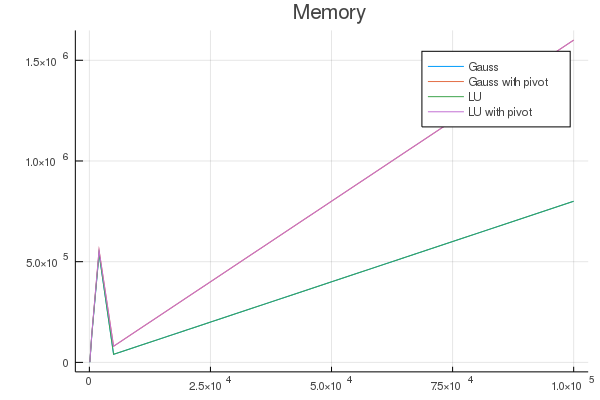
\includegraphics[width=0.8\textwidth]{memory.png}
    \caption{Wykres pamięci}
\end{figure}

\begin{figure}
  \centering
    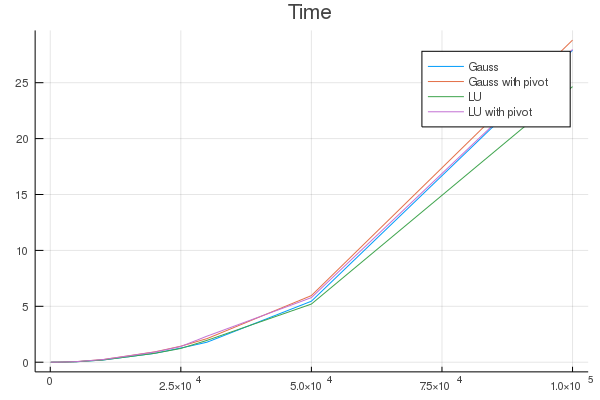
\includegraphics[width=0.8\textwidth]{times.png}}
  \caption{Wykres czasu}
\end{figure}


\end{document}




